\shorthandoff{"}
\chapter{Methodik}
\label{ch:methodik}

\section{Art der Forschung}
\label{ch:methodik:art}
Im Rahmen der vorliegenden Master-Thesis wurde eine quantitative Forschungsarbeit in Form eines Experiments mit einer anschließenden Fallstudie durchgeführt. In diesem Kontext erfolgte die Entwicklung eines Empfehlungssystems, welches sowohl uni- als auch bilaterale Vorschläge zur Besetzung offener Projektpositionen erzeugte. Für beide Ansätze wurden dieselben Projektbeschreibungen und Mitarbeiter als Eingabe verwendet. Die beiden Empfehlungsverfahren unterschieden sich lediglich in der Art, in welcher sie die vorhandenen Angestellten für die eingegebenen Stellen sortierten.

An der Fallstudie nahmen sowohl Projektmanager als auch -mitarbeiter teil. Die Angestellten erhielten Übersichten über vorausgewählte Projektpositionen und bewerteten auf einer vordefinierten Skala, wie zufrieden sie mit einer Tätigkeit auf diesen Stellen wären. Anschließend wurde überprüft, ob der bilaterale Empfehlungsansatz die Angestellten im Vergleich zur unilateralen Variante für die Stellen höher positionierte, bei welchen diese eine hohe Zufriedenheit erwarteten bzw. niedriger positionierte, wenn diese eine geringe Zufriedenheit prognostizierten.

Die Projektmanager erhielten die fünf am höchsten positionierten Mitarbeiter jedes Empfehlungsansatzes für die vorausgewählten Projektpositionen in Form von Listen. Hierbei wurde nicht vermerkt, welche Vorschläge über den uni- bzw. den bilateralen Ansatz erzeugt wurden. Die Projektmanager bewerteten auf einer vordefinierten Skala, von den Mitarbeitern welcher Liste sie eine höhere Arbeitsleistung für die jeweiligen Stellen erwarten. Anschließend wurde evaluiert, ob sie die erwartete Arbeitsleistung der vorgeschlagenen Angestellten des bilateralen Ansatzes im Vergleich zur unilateralen Variante als höher einschätzten.

Die vorliegende Master-Thesis fokussierte ausschließlich den komplementären \ac{PEFit} auf Facetten-Ebene. Hierbei wurden einzig die für die offenen Projektpositionen benötigten Kompetenzen zur Bestimmung der Kongruenz herangezogen. Weitere Faktoren wie Kundennamen oder Branchen fanden keine Berücksichtigung. Im Sinne des ergänzenden \acp{PEFit} wurde vorausgesetzt, dass eine grundlegende Überprüfung der Konformität der Werte von Mitarbeitern und Unternehmen bzw. Projekttätigkeiten bereits vor Anstellung der Arbeitnehmer stattfand.

Durchgeführt wurden das Experiment und die Fallstudie mit Projektmanagern und Mitarbeitern des Fachbereichs \JES der EXXETA AG mit Hauptsitz in Karlsruhe. Das Unternehmen ist spezialisiert auf IT-Beratungsleistungen und arbeitet vorrangig projektbasiert. Dementsprechend ist das Zuordnen passender Angestellter zu offenen Projektpositionen in diesem Betrieb eine häufig auftretende Aufgabe.

\section{Verwendete Daten des Unternehmens}
\label{ch:methodik:versuchsaufbau}
Die Mitarbeiter der EXXETA AG pflegen ihre Kompetenzen im Intranet des Unternehmens. Dort steht eine Liste mit \anzFaehigkeiten Fähigkeiten, wie beispielsweise "Java", "DSGVO" und "Digitale Transformation", zur Verfügung. Diese können die Angestellten über die in Abbildung \ref{fig:methodik:versuchsaufbau:daten:abb1} dargestellte Skala bewerten.

\begin{figure}[h]
	\centering
	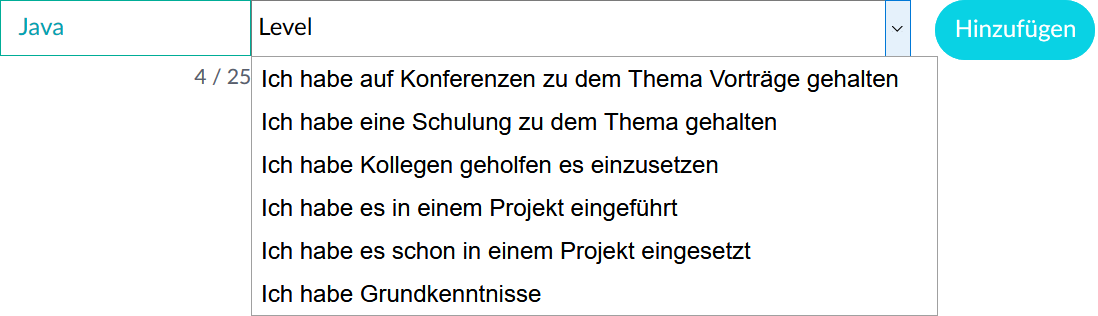
\includegraphics[width=1\textwidth]{gfx/skill-level.png}
	\caption{Hinzufügen einer Fähigkeit mit Angabe des entsprechenden Kenntnisniveaus im Intranet der EXXETA AG}
	\label{fig:methodik:versuchsaufbau:daten:abb1}
\end{figure}

Aufgrund der klaren Beschreibungen der einzelnen Stufen in Abbildung \ref{fig:methodik:versuchsaufbau:daten:abb1} konnte der in Kapitel \ref{ch:empfehlungssysteme:cf:speicherbasiert} angesprochene Bias bei der Selbsteinschätzung weitgehend ausgeschlossen werden. Außerdem war es in der vorliegenden Problemstellung gut möglich, dass einzelne Mitarbeiter ihre Kompetenzen bewusst besser oder schlechter bewerteten als andere Kollegen, da sie beispielsweise über eine längere Berufserfahrung verfügen. Aus diesen Gründen wurde bei der Empfehlungsbestimmung auf eine Mittelwert-Zentrierung verzichtet.

Damit Projektmanager Vorschläge von einem Empfehlungssystem erhalten können, müssen sie die für offene Projektpositionen nachgefragten Fähigkeiten mitsamt der benötigten Kenntnisniveaus festlegen. Die relevanten Kompetenzen bestimmen die Verantwortlichen in der Regel anhand eingehender Projektanfragen, welche Kunden in unstrukturierter Form, beispielsweise per Telefon oder E-Mail, einreichen. Derartige Anfragen werden täglich in großer Zahl bearbeitet. Daher wurde es für den praktischen Einsatz als sehr umständlich bewertet, wenn Verantwortliche für jede Projektanfrage sämtliche Fähigkeiten auf einer sechsstufigen Skala bewerten müssen. Aus diesem Grund wurden die Kompetenzniveaus aus Abbildung \ref{fig:methodik:versuchsaufbau:daten:abb1} bei der Spezifikation offener Projektpositionen auf die in Tabelle \ref{tbl:methodik:versuchsaufbau:systemarchitektur:matrixservice:tbl1} dargestellten Kompetenzniveaus vereinfacht. Bei der Definition der zur Evaluation benötigten Stellenprofile konnte für jede Fähigkeit eine der beiden Abstufungen "Grundkenntnisse" und "Fortgeschritten" angeben werden. Die Priorisierung der Kompetenzen über diese Abstufungen wurde gemäß Kapitel \ref{ch:personEnvironmentFit:wichtigkeiten} als Ausdruck von Wichtigkeiten seitens der Projektmanager betrachtet.

\begin{table}[h]
	\centering
	\begin{tabularx}{\textwidth}{c|X}
		\textbf{Kompetenzniveau} & \textbf{Bewertung im Intranet}\\
		\hline
		Keine Kenntnisse & Nicht angegeben\\
		\hline
		& Ich habe Grundkenntnisse\\
		Grundkenntnisse & Ich habe es schon in einem Projekt eingesetzt\\
		& Ich habe es in einem Projekt eingeführt\\
		\hline
		& Ich habe Kollegen geholfen es einzusetzen\\
		Fortgeschritten & Ich habe eine Schulung zu dem Thema gehalten\\
		& Ich habe auf Konferenzen zu dem Thema Vorträge gehalten\\
		\hline
	\end{tabularx}
	\caption{Vereinfachung der im Intranet hinterlegten Kompetenzniveaus}
	\label{tbl:methodik:versuchsaufbau:systemarchitektur:matrixservice:tbl1}
\end{table}

Die EXXETA AG hat zum Zeitpunkt der Durchführung des Experiments keine Präferenzen ihrer Mitarbeiter bezüglich deren Kompetenzen erhoben. Um die Wünsche der Angestellten ebenfalls in die Empfehlungsprozess einzubeziehen, wurde daher im Rahmen dieser Master-Thesis eine Umfrage durchgeführt. Die 45 Mitarbeiter des Bereichs \JES erhielten zu diesem Zweck einen Fragebogen mit den \anzFaehigkeiten im Intranet hinterlegten Fähigkeiten und wurden gebeten, für sämtliche Kompetenzen über einen booleschen Wert auszudrücken, ob sie diese gerne in Projekten anwenden möchten. Sie konnten dabei sowohl bereits beherrschte Fähigkeiten auswählen als auch Kompetenzen, welche diese zukünftig erst erlernen bzw. erstmals einsetzen möchten. Ein Auszug aus dem Fragebogen ist in Abbildung \ref{fig:methodik:versuchsaufbau:abb1} dargestellt.

\begin{figure}[h]
	\centering
	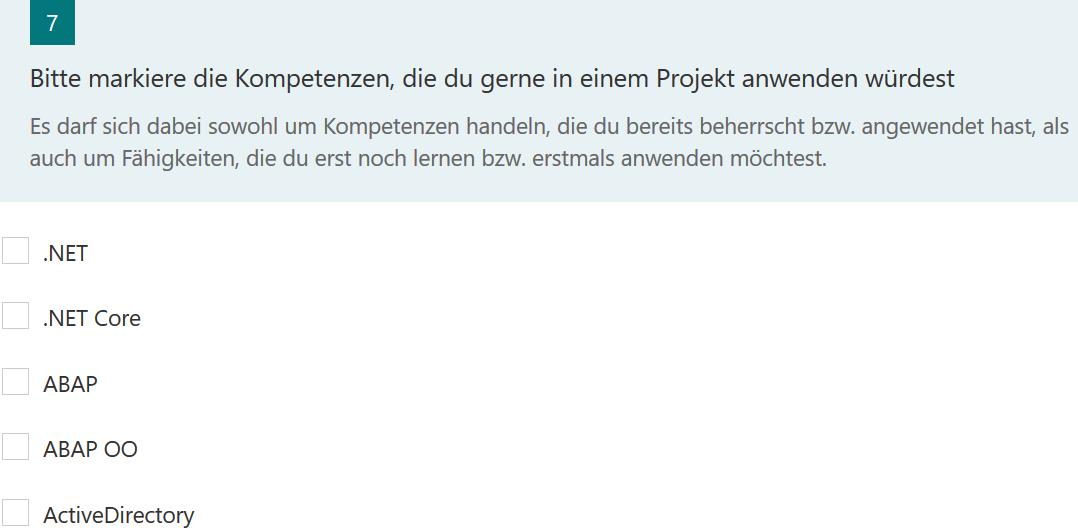
\includegraphics[width=1\textwidth]{gfx/Umfage_Faehigkeiten.png}
	\caption{Auszug aus der Umfrage zur Erhebung der Mitarbeiter-Präferenzen}
	\label{fig:methodik:versuchsaufbau:abb1}
\end{figure}

Die Kompetenzbewertungen der Mitarbeiter und deren Präferenzen dienten im Experiment als Datengrundlage für ein neu entwickeltes, hybrides Empfehlungssystem.

\section{Aufbau des hybriden Empfehlungssystems}
\label{ch:methodik:versuchsaufbau:systemarchitektur}
Das im Rahmen dieser Master-Thesis implementierte Empfehlungssystem basierte auf einer Microservice-Architektur, welche aus drei Diensten und einem Pufferspeicher bestand. Um die Funktionsweisen und Rückgaben der verschiedenen Komponenten des Systems anhand von Beispielen zu erläutern, werden die Mitarbeiter und Kompetenzbewertungen aus Tabelle \ref{tbl:empfehlungssysteme:arbeitsweise:tbl1} verwendet. Dabei wird festgelegt, dass Jane Doe und Max Muster bzw. John Doe und Erika Muster in jeweils einem Team des Fachbereichs \JES tätig sind. Zusätzlich wird angenommen, dass die Mitarbeiter die Kompetenzen aus Tabelle \ref{tbl:methodik:versuchsaufbau:systemarchitektur:tbl1} präferieren.

\begin{table}[h]
	\centering
	\begin{tabular}{c|c}
		\textbf{Nutzer} & \textbf{Präferierte Fähigkeiten}\\
		\hline
		Jane D.     & HDFS\\
		John D.     & Python, HDFS\\
		Erika M.    & MySQL, Python\\
		Max M.      & HDFS, MySQL
	\end{tabular}
	\caption{Präferierte Fähigkeiten der Beispielnutzer}
	\label{tbl:methodik:versuchsaufbau:systemarchitektur:tbl1}
\end{table}

Sämtliche Komponenten der Microservice-Architektur wurden in Form von Docker-Containern ausgeliefert und über Docker Compose orchestriert. Die Dienste kommunizierten untereinander über HTTP. Abbildung \ref{fig:methodik:systemarchitekturn:abb1} zeigt einen Überblick über die Systemarchitektur.

\begin{figure}[h]
	\centering
	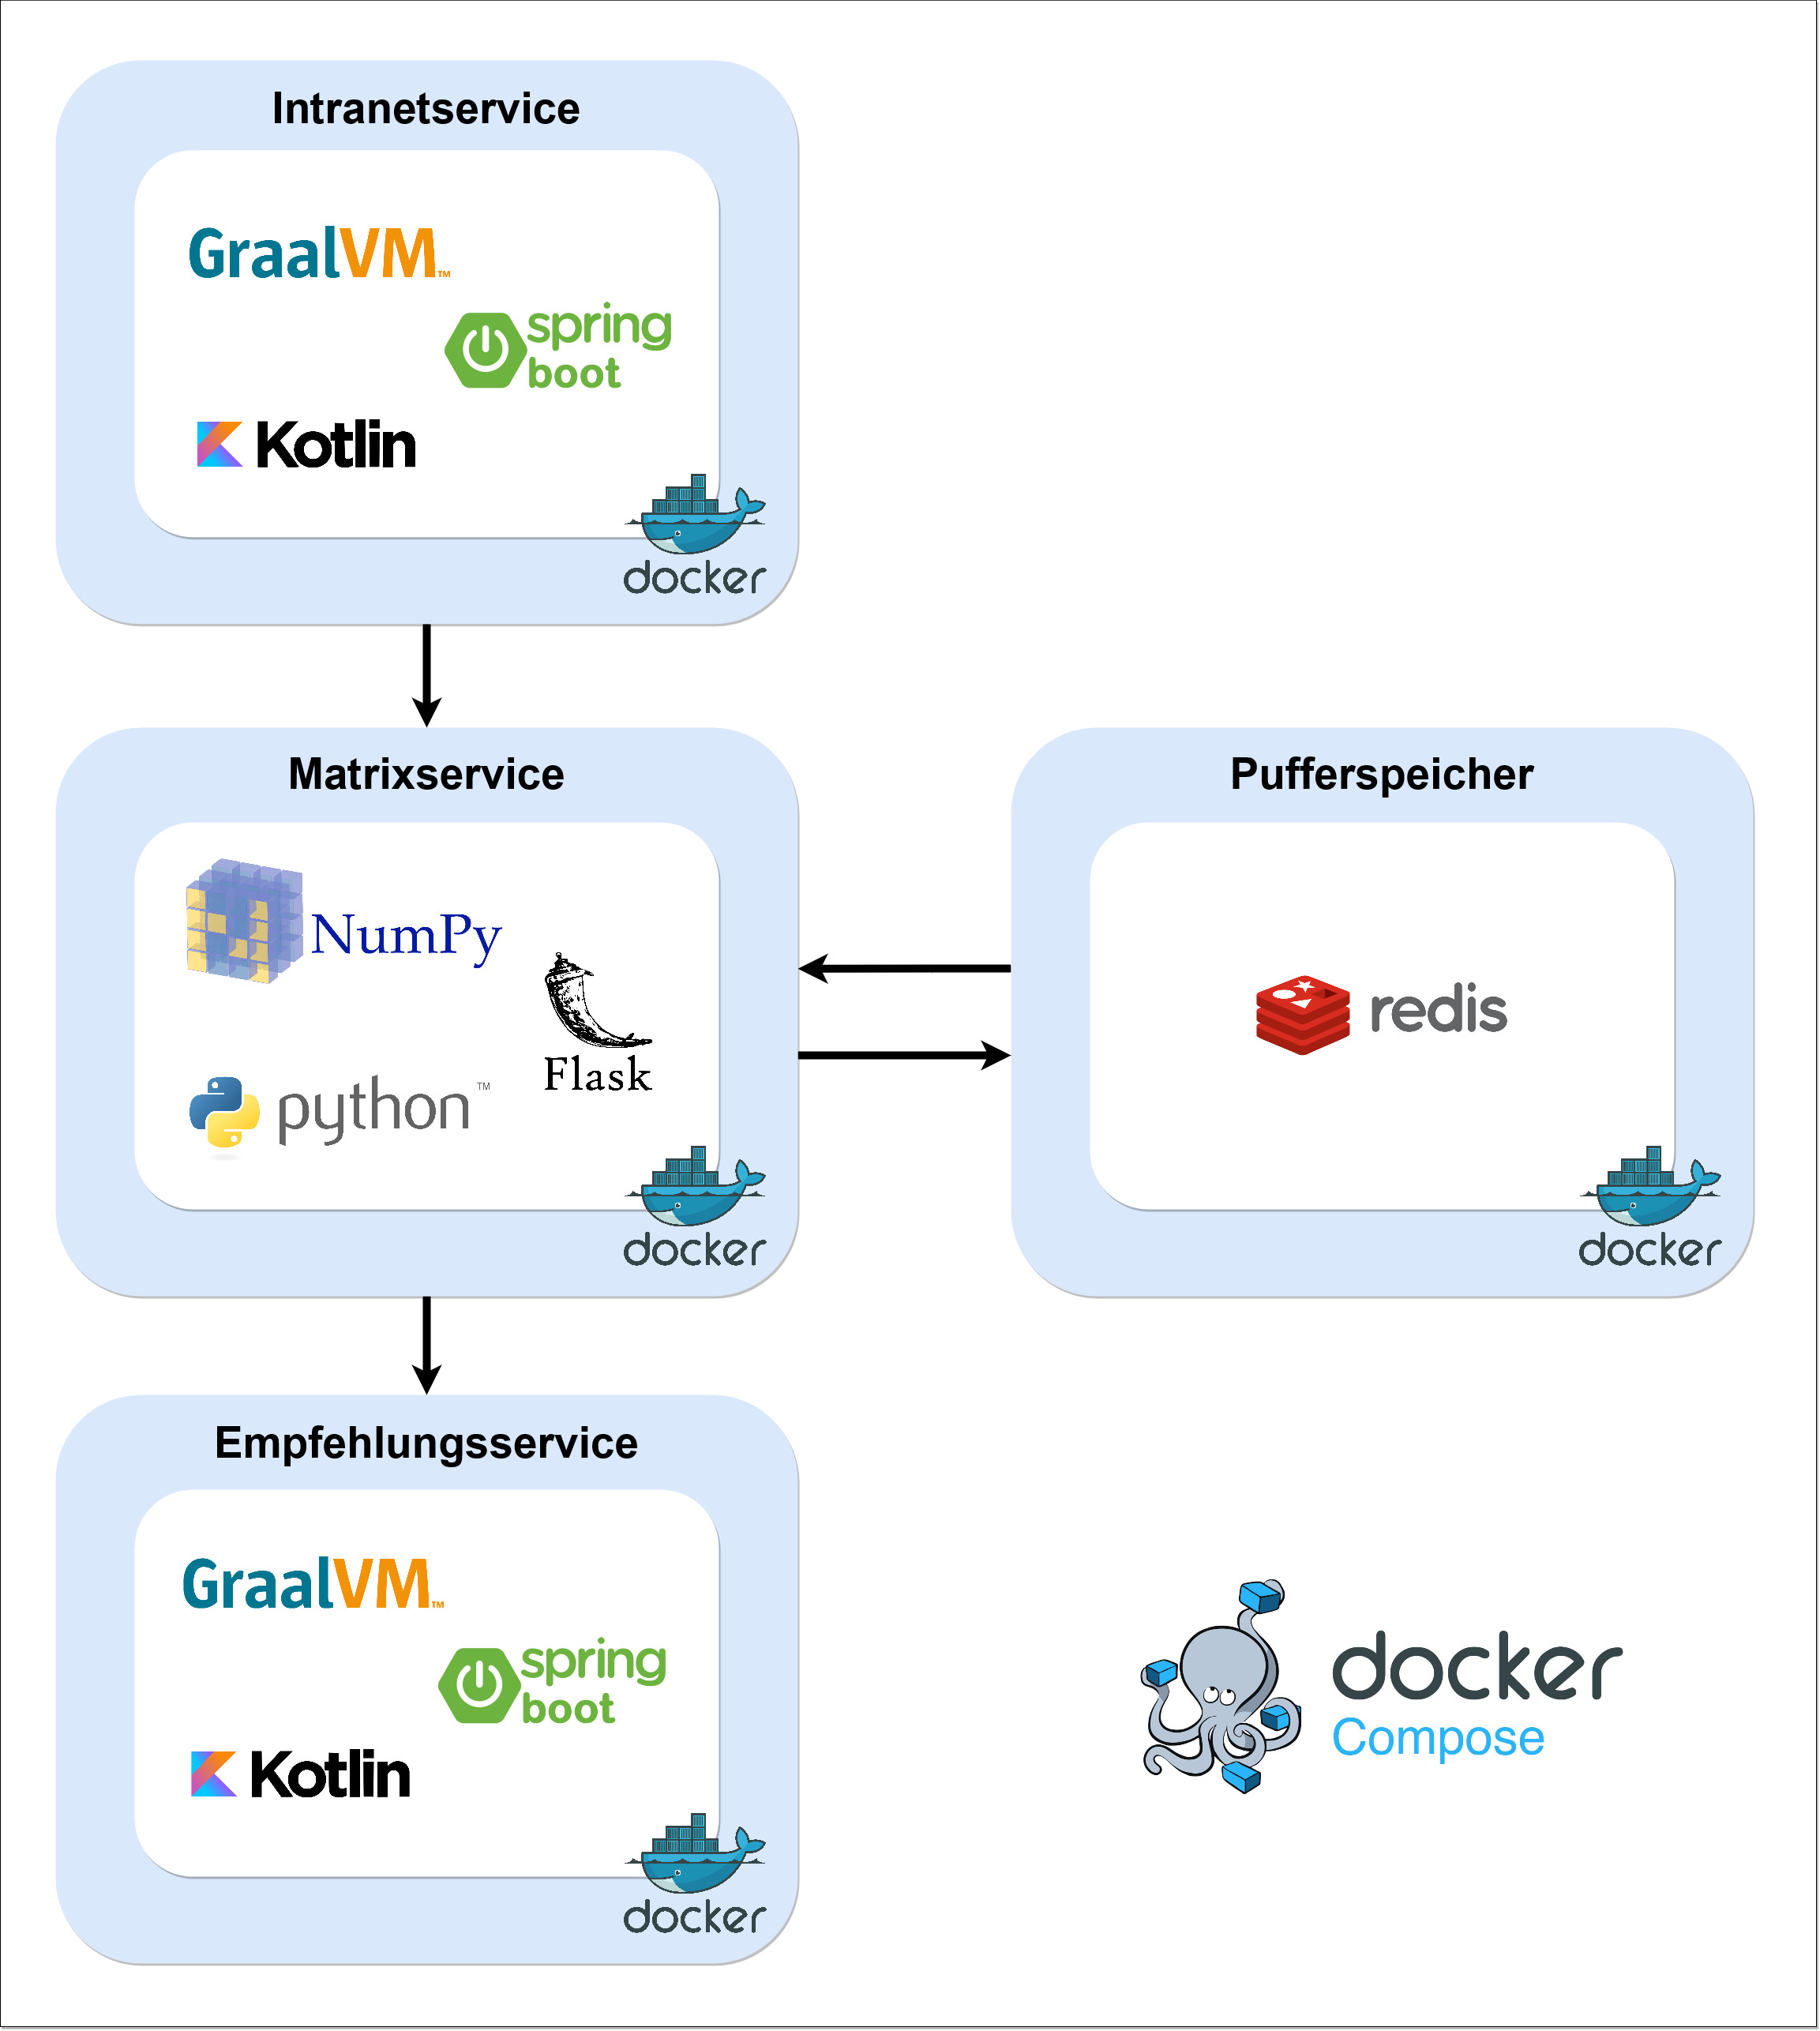
\includegraphics[width=1\textwidth]{gfx/ArchitekturMitLinie.jpg}
	\caption{Systemarchitektur des hybriden Empfehlungssystems}
	\label{fig:methodik:systemarchitekturn:abb1}
\end{figure}

Beim oben in Abbildung \ref{fig:methodik:systemarchitekturn:abb1} dargestellten Intranetservice handelte es sich um einen Dienst, welcher im Rahmen des Experiments das Intranet der EXXETA AG simulierte.

\subsection{Intranetservice}
\label{ch:methodik:versuchsaufbau:systemarchitektur:intranetservice}
Das Intranet der EXXETA AG bietet eine REST-Schnittstelle, welche Informationen über sämtliche Mitarbeiter des Unternehmens in Form von JSON bereitstellt. Über diese können die Kompetenzbewertungen und die Teamzuordnungen der Angestellten ermittelt werden. Einzelne Mitarbeiter sind dabei eindeutig über ihre E-Mail-Adresse identifizierbar.

Für die vorliegende Problemstellung wurden nicht die Daten aller Angestellten des Unternehmens benötigt. Der Empfehlungsalgorithmus griff ausschließlich auf die Informationen von denjenigen Mitarbeitern zurück, welche im Rahmen der Umfrage Präferenzen bezüglich eingesetzter Kompetenzen spezifiziert hatten.

Die Aufgabe des Intranetservices bestand darin, die Rückgabe der Schnittstelle des Intranets der EXXETA AG mit den erhobenen Präferenzen der Umfrage zu kombinieren. Außerdem wurden sämtliche nicht benötigten Informationen und Mitarbeiter zu Gunsten der Datensparsamkeit entfernt. Listing \ref{qc:methodik:versuchsaufbau:daten:qc1} zeigt einen beispielhaften Auszug aus der Rückgabe des Intranetservices.

%\begin{minipage}{\linewidth}
\lstinputlisting[
language=json,
caption=Beispiel für die Rückgabe des Intranetservices (Auszug),
captionpos=b,
label=qc:methodik:versuchsaufbau:daten:qc1
]{gfx/john.json}
%\end{minipage}

Die Implementierung des Intranetservices erfolgte in der Programmiersprache Kotlin. Als Framework wurde Spring Boot in Kombination mit dem GraalVM Native Image-Compiler verwendet, welcher die Startzeit und den benötigten Arbeitsspeicher des Dienstes stark reduzierte.

Die Daten des Intranetservices dienten als Eingabe für den Matrixservice, welcher zur Optimierung der Empfehlungsbestimmung die Sparsity- und Kaltstart-Problematik löste.

\subsection{Matrixservice}
\label{ch:methodik:versuchsaufbau:systemarchitektur:matrixservice}
Der Matrixservice basierte auf der Datenstruktur eines Graphen. Hierbei wurden die Mitarbeiter der EXXETA AG und deren Fähigkeiten in Form von Knoten dargestellt. Zur Lösung des Sparsity Problems kam der speicherbasierte Algorithmus von Katz zur Anwendung. Da die Anwendung auch über die Master-Thesis hinaus im Unternehmen zum Einsatz kommen soll, wurde insbesondere die Langlebigkeit des Verfahrens als vorteilhaft gegenüber modellbasierten Methoden bewertet. Sollten sich nach Durchführung des Experiments Daten im Unternehmen verändern oder neue Kompetenzen im Intranet hinzugefügt werden, ist das Empfehlungssystem im Gegensatz zu modellbasierten Methoden weiterhin ohne zusätzlichen manuellen Aufwand im Betrieb einsetzbar.

Im Intranet der EXXETA AG war zu beobachten, dass einige Mitarbeiter keine einzige Fähigkeit beurteilt hatten. Hierbei handelte es sich beispielsweise um neue Angestellte oder Mitarbeiter, welche bereits seit längerer Zeit ausgelastet waren und daher ihre Kompetenzen noch nicht gepflegt hatten. Diese Angestellten wären folglich im Graphen über keine Kompetenz mit keiner anderen Person verbunden worden. Somit würde ein Kaltstart bei der Empfehlungsbestimmung entstehen.

Um diesem vorzubeugen, wurden zusätzlich zu den Fähigkeiten der Mitarbeiter auch deren Teamzuordnungen in Form eines hybriden Ansatzes beachtet. Damit waren stets sämtliche Mitarbeiter des Bereichs \JES über den Abteilungsleiter bzw. alle Angestellten der EXXETA AG über den Vorstand miteinander verbunden. Die Vorgehensweise hatte zusätzlich den Vorteil, dass die Kompetenzen eines Zielnutzers bei Berechnung des Algorithmus feingranular besser bewertet wurden, wenn dessen direkte Kollegen ähnliche Fähigkeiten beherrschten. Dieser Ansatz wurde für die EXXETA AG als sinnvoll bewertet, da dort in der Regel Mitarbeiter mit vergleichbarem fachlichem Hintergrund in einem Team tätig sind. Auch die Teammanager sind fachliche Führungskräfte, deren Fähigkeiten meist weitgehend repräsentativ für ihre Mitarbeiter sind.

Um eine weitere Erhöhung der Laufzeit des algorithmisch komplexen Verfahrens von Katz zu vermeiden, wurden die Teams nicht als zusätzliche Knoten in den Graphen eingefügt. Die Beziehungen wurden stattdessen über direkte Kanten zwischen Kollegen dargestellt. Das Kantengewicht zwischen zwei Teammitgliedern bzw. einem Angestellten zu seinem Manager wurde auf \teamgewichtString festgelegt. Die Verwendung dieses Wertes bezog die Teamzugehörigkeit schwach in die Berechnung mit ein, gewichtete hohe individuelle Kompetenzbewertungen jedoch weiterhin stärker.

Abbildung \ref{fig:methodik:versuchsaufbau:unilateral:abb1} zeigt die Darstellung der Kompetenzen und die Teamzuordnungen der Beispielangestellten in Form eines Graphen.

\begin{figure}[h]
	\centering	
	\begin{tikzpicture}[node distance={31mm}, thick, main/.style = {draw, circle}] 
		\node[main, fill=itemcolor] (MongoDB) {$MongoDB$}; 
		\node[main, fill=itemcolor] (Python) [below right of=MongoDB] {$Python$}; 
		\node[main, fill=itemcolor] (MySQL) [above right of=Python] {$MySQL$}; 
		\node[main, fill=itemcolor] (Java) [below right of=MySQL] {$Java$}; 
		\node[main, fill=itemcolor] (HDFS) [above right of=Java] {$HDFS$}; 
		\node[main, fill=itemcolor] (Spark) [below right of=HDFS] {$Spark$};
		
		\node[main, fill=usercolor] (Jane) [above right of=MongoDB] {$Jane D.$}; 
		\node[main, fill=usercolor] (John) [above left of=HDFS] {$John D.$}; 
		\node[main, fill=usercolor] (Max) [below of=MySQL] {$Max M.$};
		\node[main, fill=usercolor] (Erika) [above right of=HDFS] {$Erika M.$}; 
		
		\draw (Jane) -- node[midway, right] {4} (Python);
		\draw (Jane) -- node[midway, above] {3} (MySQL);
		\draw (Jane) -- node[midway, above] {3} (MongoDB);
		\draw (Jane) -- node[midway, left] {1} (Max);
		
		\draw (John) -- node[midway, right] {1} (HDFS);		
		\draw (John) -- node[midway, right] {3} (Java);
		\draw (John) -- node[midway, above] {2} (MySQL);
		\draw (John) -- node[midway, above] {1} (Erika);
		
		%\path (Erika) edge[bend right=10] node[midway, right] {5} (HDFS); 
		\draw (Erika) -- node[midway, above] {5} (HDFS);
		\draw (Erika) -- node[midway, right] {3} (Spark);
		
		\draw (Max) -- node[midway, above] {2} (Java);
		\draw (Max) -- node[midway, above] {3} (Python);
		\draw (Max) -- node[midway, right] {1} (MySQL);
	\end{tikzpicture}
	
	\caption{Graph aus Abbildung \ref{fig:empfehlungssysteme:cf:speicherbasiert:abb2} mit zusätzlicher Teamzuordnung}
	\label{fig:methodik:versuchsaufbau:unilateral:abb1}
\end{figure}

Die in der Datenstruktur eines Graphen angeordneten Daten der Mitarbeiter dienten als Grundlage zur Berechnung des Katz-Algorithmus anhand von Gleichung \ref{frml:methodik:versuchsaufbau:systemarchitektur:matrixservice:formel1}, welche in Kapitel \ref{ch:empfehlungssysteme:cf:speicherbasiert} vorgestellt wurde.
\begin{equation}
	(I - \beta * M)^{-1} - I
	\label{frml:methodik:versuchsaufbau:systemarchitektur:matrixservice:formel1}
\end{equation}
Im Matrixservice wurde der Wert von $\beta$ über Gleichung \ref{frml:methodik:versuchsaufbau:grundlegend:formel1} bestimmt.
\begin{equation}
	\beta = \frac{1/\lambda}{\nenner}
	\label{frml:methodik:versuchsaufbau:grundlegend:formel1}
\end{equation}
Durch das in Gleichung \ref{frml:methodik:versuchsaufbau:grundlegend:formel1} dargestellte Vorgehen wurde sichergestellt, dass $\beta$ auch bei sich ändernder Datenlage die Größe von $1/\lambda$ nicht überschreitet. Wie in Kapitel \ref{ch:empfehlungssysteme:cf:speicherbasiert} erläutert, entspricht $\lambda$ dem größten Eigenwert der Adjazenzmatrix $M$ des Graphen.%Aufgrund der Division durch \nenner war $\beta$ stets so groß, dass von einem Zielnutzer weit entfernte Knoten in die Berechnung einbezogen wurden und nahe Fähigkeiten zusätzlich stark gewichtet werden.

Wie in Kapitel \ref{ch:empfehlungssysteme:cf:speicherbasiert} beschrieben, ändern sich bei Berechnung des Verfahrens von Katz die Fähigkeitsbewertungen. Allerdings befinden sich die Beurteilungen, welche ursprünglich einem gemeinsamen Kompetenzniveau entsprachen, auch nach Berechnung des Algorithmus auf einem vergleichbaren Niveau. Die Werte innerhalb eines Kompetenzbereichs sind lediglich feingranular unterschiedlich. Dieses Phänomen ist in Tabelle \ref{tbl:methodik:versuchsaufbau:unilateral:tbl1} zu beobachten. Dort sind die Bewertungen der Fähigkeit MySQL aus Abbildung \ref{fig:methodik:versuchsaufbau:unilateral:abb1} vor und nach Berechnung des Katz-Algorithmus eingetragen. Gleiche Kompetenzniveaus sind in Tabelle \ref{tbl:methodik:versuchsaufbau:unilateral:tbl1} durch einheitliche Hintergrundfarben gekennzeichnet.

\begin{table}[h]
	\centering
	\begin{tabular}{c|c|c|c}
		\textbf{Name} & \textbf{Kompetenzniveau} & \textbf{Original-Bewertung} & \textbf{Matrix-Ergebnis} \\
		\hline
		\rowcolor{exxetagray}Erika M. & Keine Kenntnisse & 0 & 0.42\\
		\hline
		\rowcolor{itemcolor}Max M.    & Grundkenntnisse  & 1 & 1.32\\
		\rowcolor{itemcolor}John D.   & Grundkenntnisse  & 2 & 0.92\\
		\rowcolor{itemcolor}Jane D.   & Grundkenntnisse  & 3 & 2.10
	\end{tabular}
	\caption{Ergebnisse des Katz-Algorithmus für die Kompetenz MySQL im Graphen aus Abbildung \ref{fig:methodik:versuchsaufbau:unilateral:abb1}}
	\label{tbl:methodik:versuchsaufbau:unilateral:tbl1}
\end{table}

Wie in Tabelle \ref{tbl:methodik:versuchsaufbau:unilateral:tbl1} zu erkennen, haben Max Muster, Jane und John Doe auch nach Berechnung des Katz-Algorithmus vergleichbare Bewertungen. Es kann interpretiert werden, dass sich die drei Beispielangestellten ähnlich gut mit MySQL auskennen, Jane Doe die Fähigkeit jedoch wenig besser beherrscht als ihre beiden Kollegen. Die Ergebnisse der letzten Spalte von Tabelle \ref{tbl:methodik:versuchsaufbau:unilateral:tbl1} wurden als unilateraler Empfehlungswert betrachtet. Der Empfehlungsservice benötigte diesen Wert zu einem späteren Zeitpunkt zur Bestimmung von Vorschlägen.

Es wurde davon ausgegangen, dass die Präferenz eines Mitarbeiters für eine Fähigkeit seine Motivation erhöht und dessen Kompetenzbewertung daher gegenüber den anderen Angestellten innerhalb seines Kompetenzniveaus zunimmt. Aus diesem Grund bestimmte der Matrixservice in einem weiteren Rechenschritt für jede Fähigkeit die höchste Bewertung innerhalb jedes der drei Kompetenzniveaus aus Tabelle \ref{tbl:methodik:versuchsaufbau:systemarchitektur:matrixservice:tbl1}. Favorisierte ein Mitarbeiter eine bestimmte Fähigkeit, addierte der Dienst die höchste Bewertung des Kompetenzniveaus, auf welchem sich der Mitarbeiter befand, zu dessen Beurteilung. Durch dieses Vorgehen verblieben die Angestellten bei ihrer ursprünglichen Bewertung, wenn sie die betrachtete Kompetenz nicht präferieren. Wünschten sich mehrere Mitarbeiter die Fähigkeit im Projekt anzuwenden, erhielten sie innerhalb des Kompetenzniveaus eine höhere Positionierung. Hierbei blieb die ursprüngliche Reihenfolge der Angestellten gleich, sodass Projektmanager als ersten Vorschlag den fähigsten und zugleich motiviertesten Angestellten erhielten. Somit wurden gemäß des ergänzenden \acp{PEFit} gleichzeitig die Präferenzen von Projektmanagern und Mitarbeitern betrachtet. Die Ergebnisse des beschriebenen Rechenschritts wurden anschließend als bilateraler Empfehlungswert gespeichert. Die unilateralen und bilateralen Empfehlungswerte für die Beispielmitarbeiter sind in Tabelle \ref{tbl:methodik:versuchsaufbau:unilateral:tbl3} dargestellt.

\begin{table}[h]
	\centering
	\begin{tabular}{c|c|c|c|c|c}
		\textbf{Name} & \textbf{Niveau} & \textbf{Orig.-Bew.} & \textbf{Unil.-Empf.} & \textbf{Präferenz} & \textbf{Bil.-Empf.}\\
		\hline
		\rowcolor{exxetagray}Erika M. & Keine K. & 0 & 0.42 & Ja   & 0.84\\
		\hline
		\rowcolor{itemcolor}Max M.    & Grundk.  & 1 & 1.32 & Ja   & 3.42\\
		\rowcolor{itemcolor}John D.   & Grundk.  & 2 & 0.92 & Nein & 0.92\\
		\rowcolor{itemcolor}Jane D.   & Grundk.  & 3 & 2.10 & Nein & 2.10
	\end{tabular}
	\caption{Uni- und bilaterale Ergebnisse des Katz-Algorithmus für die Kompetenz MySQL im Graphen aus Abbildung \ref{fig:methodik:versuchsaufbau:unilateral:abb1}}
	\label{tbl:methodik:versuchsaufbau:unilateral:tbl3}
\end{table}
\newpage
In Tabelle \ref{tbl:methodik:versuchsaufbau:unilateral:tbl3} ist zu erkennen, dass sich die bilateralen Empfehlungswerte von Erika und Max Muster von ihren unilateralen Empfehlungswerten unterscheiden. Ursächlich ist, dass beide Mitarbeiter die Fähigkeit MySQL präferieren. Da Erika Muster in der Tabelle als geeignetste Mitarbeiterin auf ihrem Kompetenzniveau für die Fähigkeit MySQL betrachtet wird, verdoppelt sich ihre Beurteilung bei der Bestimmung des bilateralen Empfehlungswertes. Jane Doe ist dagegen die potentiell fähigste Angestellte mit Grundkenntnissen in MySQL. Da Max Muster diese Kompetenz präferiert, wird bei Berechnung des bilateralen Empfehlungswertes sein Ergebnis des Katz-Algorithmus zu Jane Does Resultat addiert. Durch diesen Rechenschritt befinden sich sämtliche Bewertungen der Fähigkeit MySQL auch nach Bestimmung des bilateralen Empfehlungswertes auf einem vergleichbaren Niveau. Lediglich die Reihenfolge der Mitarbeiter ist innerhalb der Kompetenzstufen verändert.

Der Matrixservice gab die uni- und bilateralen Empfehlungswerte in Form von JSON zurück. Listing \ref{qc:methodik:versuchsaufbau:daten:qc2} zeigt beispielhaft eine Ausgabe des Matrixservice, welche einen Auszug der Daten von John Doe enthält.

%\begin{minipage}{\linewidth}
\lstinputlisting[
language=json,
caption=Beispiel für die Rückgabe des Matrixservices (Auszug),
captionpos=b,
label=qc:methodik:versuchsaufbau:daten:qc2
]{gfx/john-matrix.json}
%\end{minipage}

In Listing \ref{qc:methodik:versuchsaufbau:daten:qc2} ist zu erkennen, dass jede Fähigkeit vier Attribute besaß. Die Werte von uni- bzw. bilateralLevel standen für die uni- bzw. bilateralen Empfehlungswerte. Das Attribut preference zeigte an, ob der Mitarbeiter die Kompetenz präferierte. Der Wert von originalLevel gab die originale Kompetenzbewertung des Angestellten aus dem Intranet wieder, welche den Kantengewichten im Graphen entsprachen.

Da die Berechnung des Verfahrens von Katz eine hohe algorithmische Komplexität aufweist, speicherte der Matrixservice die Ergebnisse seiner Berechnung zur effizienteren Vorschlagsbestimmung in einem Pufferspeicher zwischen. Dieses Vorgehen kombinierte die Vorteile von speicher- und modellbasierten Empfehlungsansätzen. Wie bei speicherbasierten Verfahren üblich, konnte der Matrixservice stets auf die aktuellen Daten des Unternehmens zurückgreifen. Durch die Zwischenspeicherung der Ergebnisse wurde gleichzeitig eine bei modellbasierten Verfahren zu erwartende Effizienz bei der Empfehlungsgenerierung erzielt.

Die Implementierung des Matrixservices erfolgte in der Programmiersprache Python. Eingesetzt wurden dabei das Framework Flask und das Paket Numpy, welches die Matrixberechnungen unterstützte. Als Pufferspeicher kam der Schlüssel-Wert-Speicher Redis zum Einsatz.

Die finale Empfehlungsbestimmung anhand der Ausgabe des Matrixservices erfolgte abschließend im Empfehlungsservice.

\subsection{Empfehlungsservice}
\label{ch:methodik:versuchsaufbau:systemarchitektur:empfehlungsservice}
Der Empfehlungsservice enthielt eine Schnittstelle, über welche Projektmanager die für offene Projektpositionen benötigten Fähigkeiten eingeben konnten. Wie in Listing \ref{qc:methodik:versuchsaufbau:systemarchitektur:empfehlungsservice:qc1} dargestellt, mussten diese den Namen jeder Kompetenz angeben und das gesuchte Fähigkeitsniveau über das boolesche Attribut expert spezifizieren.

%\begin{minipage}{\linewidth}
\lstinputlisting[
language=json,
caption=Beispiel für eine Eingabe in den Empfehlungsservice,
captionpos=b,
label=qc:methodik:versuchsaufbau:systemarchitektur:empfehlungsservice:qc1
]{gfx/project-input.json}
%\end{minipage}

Bei der unilateralen Vorschlagsgenerierung bestimmte der Empfehlungsservice gemäß des Anforderungen-Fähigkeiten Fits ausschließlich Angestellte, welche die höchste Eignung für die Ansprüche des Projektmanagers aufweisen konnten. Hierbei wurde angenommen, dass die Verantwortlichen anstreben, offene Projektpositionen mit fachlich optimal passenden Mitarbeitern zu besetzen und folglich sowohl Über- als auch Unterqualifizierung ihrer Angestellten vermeiden möchten. Aus diesem Grund wurde der \ac{PEFit} anhand von Kurve B in Abbildung \ref{fig:methodik:versuchsaufbau:unilateral:abb2} über die quadrierte Differenzberechnung bestimmt.

\begin{figure}[h]
	\centering
	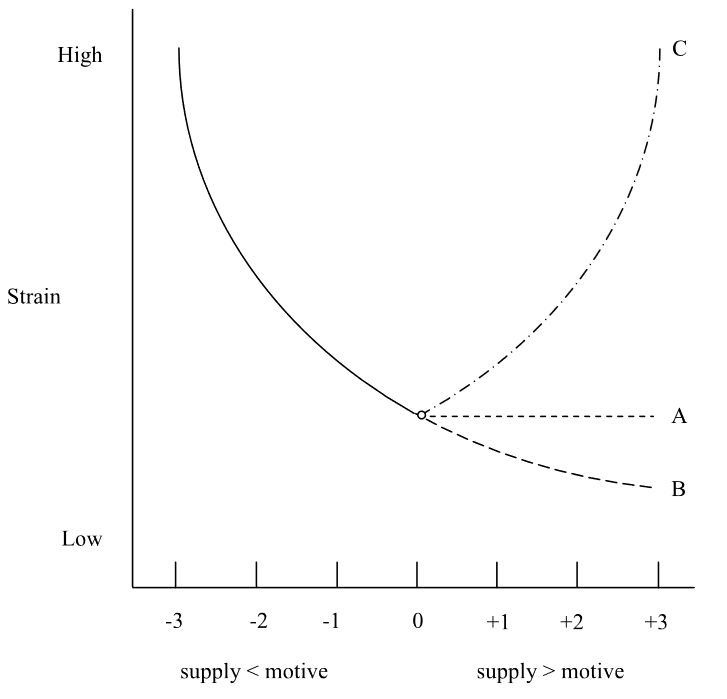
\includegraphics[width=0.75\textwidth]{gfx/ueberschuss_supply_motive.png}
	\caption[Auswirkungen eines P-E Misfits]{Auswirkungen eines P-E Misfits\\(Eigene Darstellung in Anlehnung an \cite[S. 23]{edwards:2008})}
	\label{fig:methodik:versuchsaufbau:unilateral:abb2}
\end{figure}

Würde ein Projektmanager anhand der Daten aus Tabelle \ref{tbl:methodik:versuchsaufbau:unilateral:tbl3} einen Mitarbeiter mit Grundkenntnissen in MySQL suchen, würde der Angestellte mit dem höchsten Wert im gesuchten Kompetenzbereich als geeignetster Kandidat betrachtet. Im vorliegenden Beispiel wäre somit Jane Doe die qualifizierteste Mitarbeiterin für die Suche nach einem Angestellten mit Grundkenntnissen im Umgang mit MySQL. Ihre Bewertung würde daher bei der Bestimmung des \acp{PEFit} als Nullpunkt in Abbildung \ref{fig:methodik:versuchsaufbau:unilateral:abb2} dienen.

Falls kein Mitarbeiter im gesuchten Kompetenzbereich vorhanden war, führte der Empfehlungsservice eine Ausnahmebehandlung durch. Gab es keinen passenden Kandidaten mit Grundkenntnissen in einer bestimmten Fähigkeit, wurde der am wenigsten qualifizierteste Angestellte auf fortgeschrittenem Niveau als Referenz genutzt. Konnte kein Mitarbeiter mit fortgeschrittenen Kenntnissen gefunden werden, nutzte der Empfehlungsdienst den am besten qualifizierten Kandidaten mit Grundkenntnissen als Referenz. Waren ausschließlich Mitarbeiter ohne Kenntnisse vorhanden, wurde die gesuchte Kompetenz übersprungen, da in diesem Fall kein Mitarbeiter im Graphen mit dieser Fähigkeit verbunden sein konnte und somit alle Kantengewichte \nullWert betragen mussten.

Tabelle \ref{tbl:methodik:versuchsaufbau:unilateral:tbl2} zeigt das Ergebnis der unilateralen Empfehlungsbestimmung für die Beispielmitarbeiter und das angefragte Projekt aus Listing \ref{qc:methodik:versuchsaufbau:systemarchitektur:empfehlungsservice:qc1}. Die vollständige Berechnung kann in Anhang \ref{ch:nebenrechnungen:unilateral} nachvollzogen werden.

\begin{table}[h]
	\centering
	\begin{tabular}{c|c|c}
		\textbf{Positionierung} & \textbf{Mitarbeiter} & \textbf{Abweichung}\\
		\hline
		1 & Jane D.  & 0.1\\
		2 & Max M.   & 1.6\\
		3 & John D.  & 5.9\\
		4 & Erika M. & 10.4
	\end{tabular}
	\caption{Ergebnisliste der unilateralen Empfehlungsbestimmung für eine Beispielprojektposition}
	\label{tbl:methodik:versuchsaufbau:unilateral:tbl2}
\end{table}

Die letzte Spalte in Tabelle \ref{tbl:methodik:versuchsaufbau:unilateral:tbl2} gibt die aufsummierten quadrierten Abweichungen der einzelnen Fähigkeitsbewertungen der Mitarbeiter von den bestimmten Referenzbeurteilungen an. Je kleiner die Abweichung ist, desto besser sind die Mitarbeiter folglich für die zu besetzende Projektposition geeignet. In den Ergebnissen ist zu erkennen, dass für die Stelle aus Listing \ref{qc:methodik:versuchsaufbau:systemarchitektur:empfehlungsservice:qc1} Jane Doe als geeignetste Angestellte bewertet wird.

Ähnlich zum bisher vorgestellten Vorgehen bestimmte der Empfehlungsservice auch die bilateralen Resultate. Dabei bezog der Dienst neben dem Anforderungen-Fähigkeiten Fit auch die Präferenzen der Mitarbeiter bzw. die Bedürfnisse-Angebote Kongruenz zur Bestimmung eines vollständigen \acp{PEFit} in die Berechnung mit ein. Hierbei wurden aus der Rückgabe des Matrixservice aus Listing \ref{qc:methodik:versuchsaufbau:daten:qc2} anstelle der unilateralen die bilaterale Empfehlungswerte verwendet. Durch dieses Vorgehen wurden, wie von \textcite[S. 51ff.]{edwards:1991} in Kapitel \ref{ch:personEnvironmentFit:regressionsgleichungen} gefordert, die Präferenzen von Projektmanagern und Angestellten getrennt voneinander in die Berechnung einbezogen.

Hinsichtlich der Linien aus Abbildung \ref{fig:methodik:versuchsaufbau:unilateral:abb2} wurde auch von den Mitarbeitern erwartet, dass diese Über- und Unterforderung bei der Projektarbeit vermeiden möchten. Daher wurde auch bei dieser Berechnung Kurve B über die quadrierte Differenzberechnung implementiert.

Tabelle \ref{tbl:methodik:versuchsaufbau:bilateral:tbl2} zeigt die Ergebnisse der bilateralen Empfehlungsbestimmung für die Projektposition aus Listing \ref{qc:methodik:versuchsaufbau:systemarchitektur:empfehlungsservice:qc1}. Die vollständige Berechnung kann in Anhang \ref{ch:nebenrechnungen:bilateral} nachvollzogen werden.

\begin{table}[h]
	\centering
	\begin{tabular}{c|c|c}
		\textbf{Positionierung} & \textbf{Mitarbeiter} & \textbf{Abweichung}\\
		\hline
		1 & Max M.   & 1.4\\
		2 & Jane D.  & 2.1\\
		3 & John D.  & 8.0\\
		4 & Erika M. & 9.8
	\end{tabular}
	\caption{Ergebnisliste der bilateralen Empfehlungsbestimmung für ein Beispielprojekt}
	\label{tbl:methodik:versuchsaufbau:bilateral:tbl2}
\end{table}

\newpage
In Tabelle \ref{tbl:methodik:versuchsaufbau:bilateral:tbl2} ist zu erkennen, dass Max Muster aufgrund seiner Präferenzen besser positioniert ist als zuvor in Tabelle \ref{tbl:methodik:versuchsaufbau:unilateral:tbl2}. Außerdem hat sich der Abstand von Erika Muster auf John Doe verringert.

Wie der Intranetservice wurde auch der Empfehlungsservice in der Programmiersprache Kotlin implementiert. Ebenfalls kamen das Framework Spring Boot und der GraalVM Native Image-Compiler zum Einsatz. Ein Auszug aus der Rückgabe des Empfehlungsservice für die Projektanfrage aus Listing \ref{qc:methodik:versuchsaufbau:systemarchitektur:empfehlungsservice:qc1} ist in Listing \ref{qc:methodik:versuchsaufbau:daten:qc3} dargestellt. Darin ist zu erkennen, dass für jeden Mitarbeiter die berechnete Abweichung unter der Bezeichnung recommendationValue zurückgegeben wurde. Außerdem konnte für jeden Angestellten entnommen werden, ob dieser die gesuchten Fähigkeiten präferierte und welche Bewertungen er im Intranet für die Kompetenzen abgegeben hatte.

Die Ausgaben des Empfehlungsservice dienten im Rahmen dieser Master-Thesis als Grundlage für eine Fallstudie, welche zur Beantwortung der Forschungsfrage mit Projektmanagern und Mitarbeitern des Fachbereichs \JES der EXXETA AG durchgeführt wurde.

\begin{minipage}{\linewidth}
\lstinputlisting[
language=json,
caption=Beispiel für die Rückgabe des Empfehlungsservices (Auszug),
captionpos=b,
label=qc:methodik:versuchsaufbau:daten:qc3
]{gfx/john-empfehlungsservice.json}
\end{minipage}

\section{Aufbau der Fallstudie}
\label{ch:methodik:evaluation}
Vor Durchführung der Fallstudie definierte ein Projektmanager des Fachbereichs \JES fünf beispielhafte Projektpositionen. Dieser betrachtete die Stellen als repräsentativ für häufige Kundenanfragen an die Abteilung. Abbildung \ref{fig:methodik:evaluation:abb2} zeigt die vordefinierten Projektpositionen.

\begin{figure}[h]
	\centering
	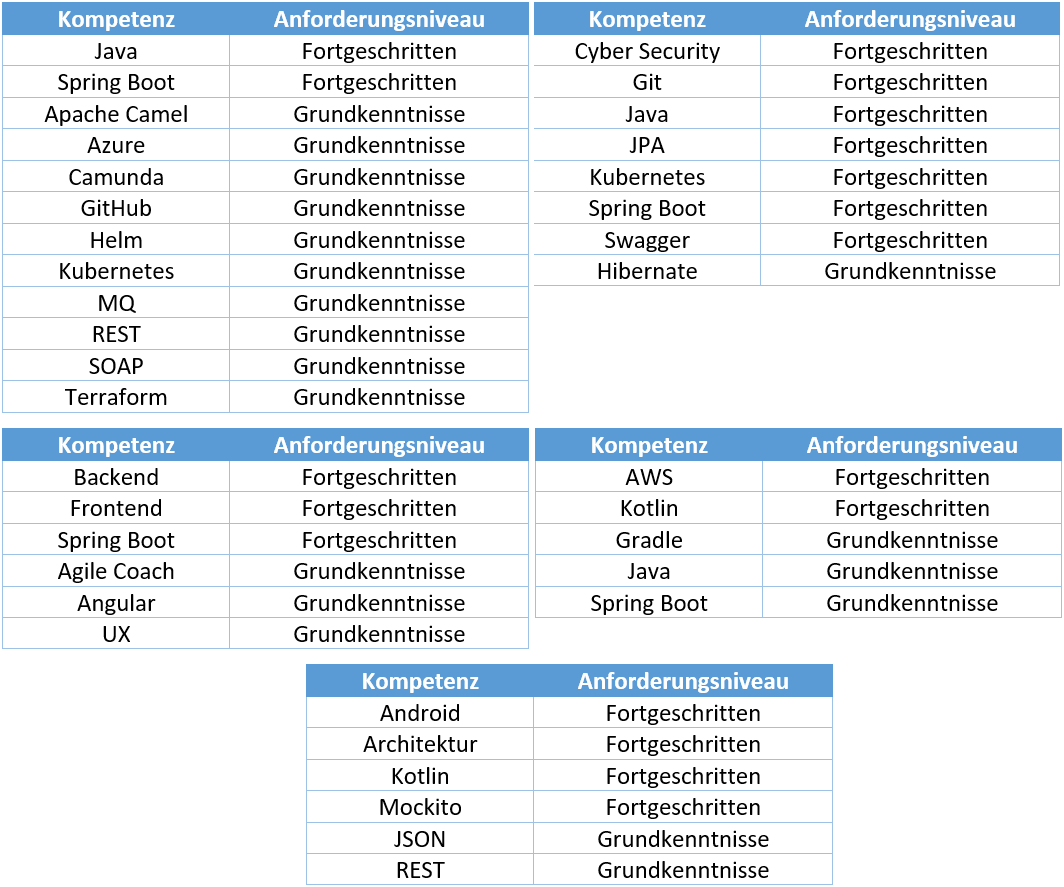
\includegraphics[width=1.0\textwidth]{gfx/Projekt.png}
	\caption{Für die Evaluation definierte Projektpositionen}
	\label{fig:methodik:evaluation:abb2}
\end{figure}

Die in Abbildung \ref{fig:methodik:evaluation:abb2} dargestellten Projektpositionen dienten als Grundlage für eine Befragung der Mitarbeiter und der Projektmanager des Bereichs \JES.

\section{Befragung der Projektmitarbeiter}
\label{ch:methodik:evaluation:mitarbeiter}
Wie anhand von Abbildung \ref{fig:methodik:versuchsaufbau:abb1} beschrieben, wurden die Mitarbeiter der EXXETA AG in einer Umfrage gebeten, ihre präferierten Kompetenzen auszuwählen. In dieser Befragung erhielten sie zusätzlich die vordefinierten Projektpositionen aus Abbildung \ref{fig:methodik:evaluation:abb2}. Hierbei sollten sie ihre Zufriedenheit mit einer Tätigkeit auf den dargestellten Projektpositionen auf einer vierstufigen Skala bewerten. Diese wurde gewählt, um neutrale Beurteilungen zu vermeiden. Abbildung \ref{fig:methodik:evaluation:abb1} zeigt einen Auszug aus der Umfrage, welchem auch die Aufgabenstellung zu entnehmen ist.

\begin{figure}[h]
	\centering
	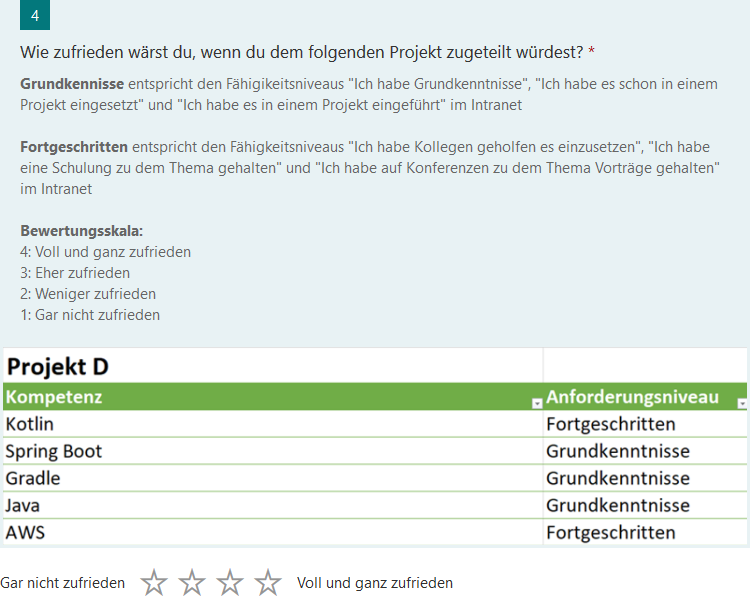
\includegraphics[width=1\textwidth]{gfx/projekt-umfrage.png}
	\caption{Bewertung eines Projektes im Fragebogen der Mitarbeiter}
	\label{fig:methodik:evaluation:abb1}
\end{figure}

Nach Abschluss der Umfrage wurde überprüft, ob das bilaterale Empfehlungssystem die Angestellten für die Projektpositionen höher positionierte, bei welchen diese eine hohe Zufriedenheit erwarteten bzw. niedriger positionierte, wenn diese eine geringe Zufriedenheit prognostizierten.

Zusätzlich wurde überprüft, wie die Angestellten einer möglichen Unterforderung bei der Projekttätigkeit gegenüber stehen. Die entsprechende Frage ist in Abbildung \ref{fig:methodik:evaluation:abb3} dargestellt.

\begin{figure}[h]
	\centering
	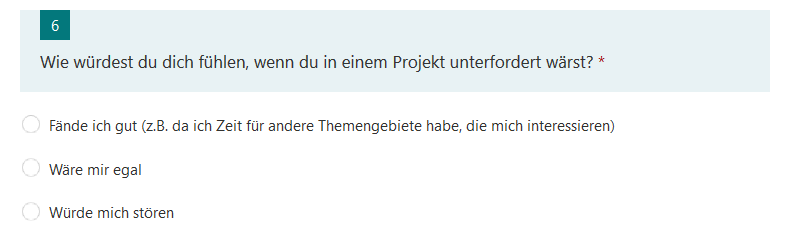
\includegraphics[width=1\textwidth]{gfx/umfrage-mitarbeiter-unterforderung.png}
	\caption{Frage zur Unterforderung der Mitarbeiter im Fragebogen der Angestellten}
	\label{fig:methodik:evaluation:abb3}
\end{figure}

Die Frage aus Abbildung \ref{fig:methodik:evaluation:abb3} diente der Überprüfung der Hypothese, dass Mitarbeiter sowohl eine Unter- als auch eine Überforderung bei der Projekttätigkeit vermeiden möchten. Diese Annahme bildete die Grundlage, Kurve B aus Abbildung \ref{fig:methodik:versuchsaufbau:unilateral:abb2} bei Bestimmung des \acp{PEFit} in Form der quadrierten Differenzberechnung zu implementieren.

\section{Befragung der Projektmanager}
\label{ch:methodik:evaluation:manager}
Neben der Befragung der Angestellten wurde eine Umfrage unter Projektmanagern durchgeführt. Diese erhielten die fünf qualifiziertesten Mitarbeiter jedes Empfehlungsansatzes für die vorausgewählten Projektpositionen in Form von Listen. Anschließend bewerteten sie auf einer vordefinierten Skala, von welchen Angestellten sie eine höhere Arbeitsleistung für die jeweiligen Stellen erwarten. Abbildung \ref{fig:methodik:evaluation:manager:abb1} zeigt auf der folgenden Seite einen Auszug aus der Befragung. Dort ist zu beobachten, dass die Projektmanager nicht erkennen konnten, welche Liste durch den unilateralen bzw. den bilateralen Empfehlungsansatz erzeugt wurde.

Im Anschluss an die Umfrage wurde evaluiert, wie die Projektmanager die erwartete Leistung der vorgeschlagenen Angestellten des bilateralen Ansatzes im Vergleich zur unilateralen Variante bewerteten.

Zusätzlich wurde auch in der Umfrage unter den Projektmanagern geprüft, wie diese mit möglicher Unterforderung ihrer Angestellten bei der Besetzung offener Projektpositionen umgehen. Die entsprechende Frage ist in Abbildung \ref{fig:methodik:evaluation:manager:abb3} dargestellt.

\begin{figure}[h]
	\centering
	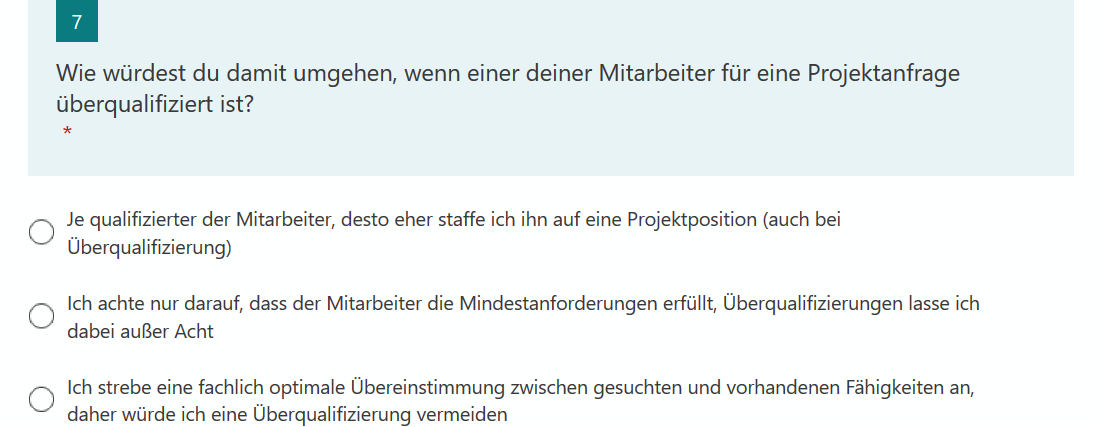
\includegraphics[width=1\textwidth]{gfx/umfrage-projektmanager-unterforderung.png}
	\caption{Frage zur Unterforderung der Mitarbeiter im Fragebogen der Projektmanager}
	\label{fig:methodik:evaluation:manager:abb3}
\end{figure}

\begin{figure}[h]
\centering
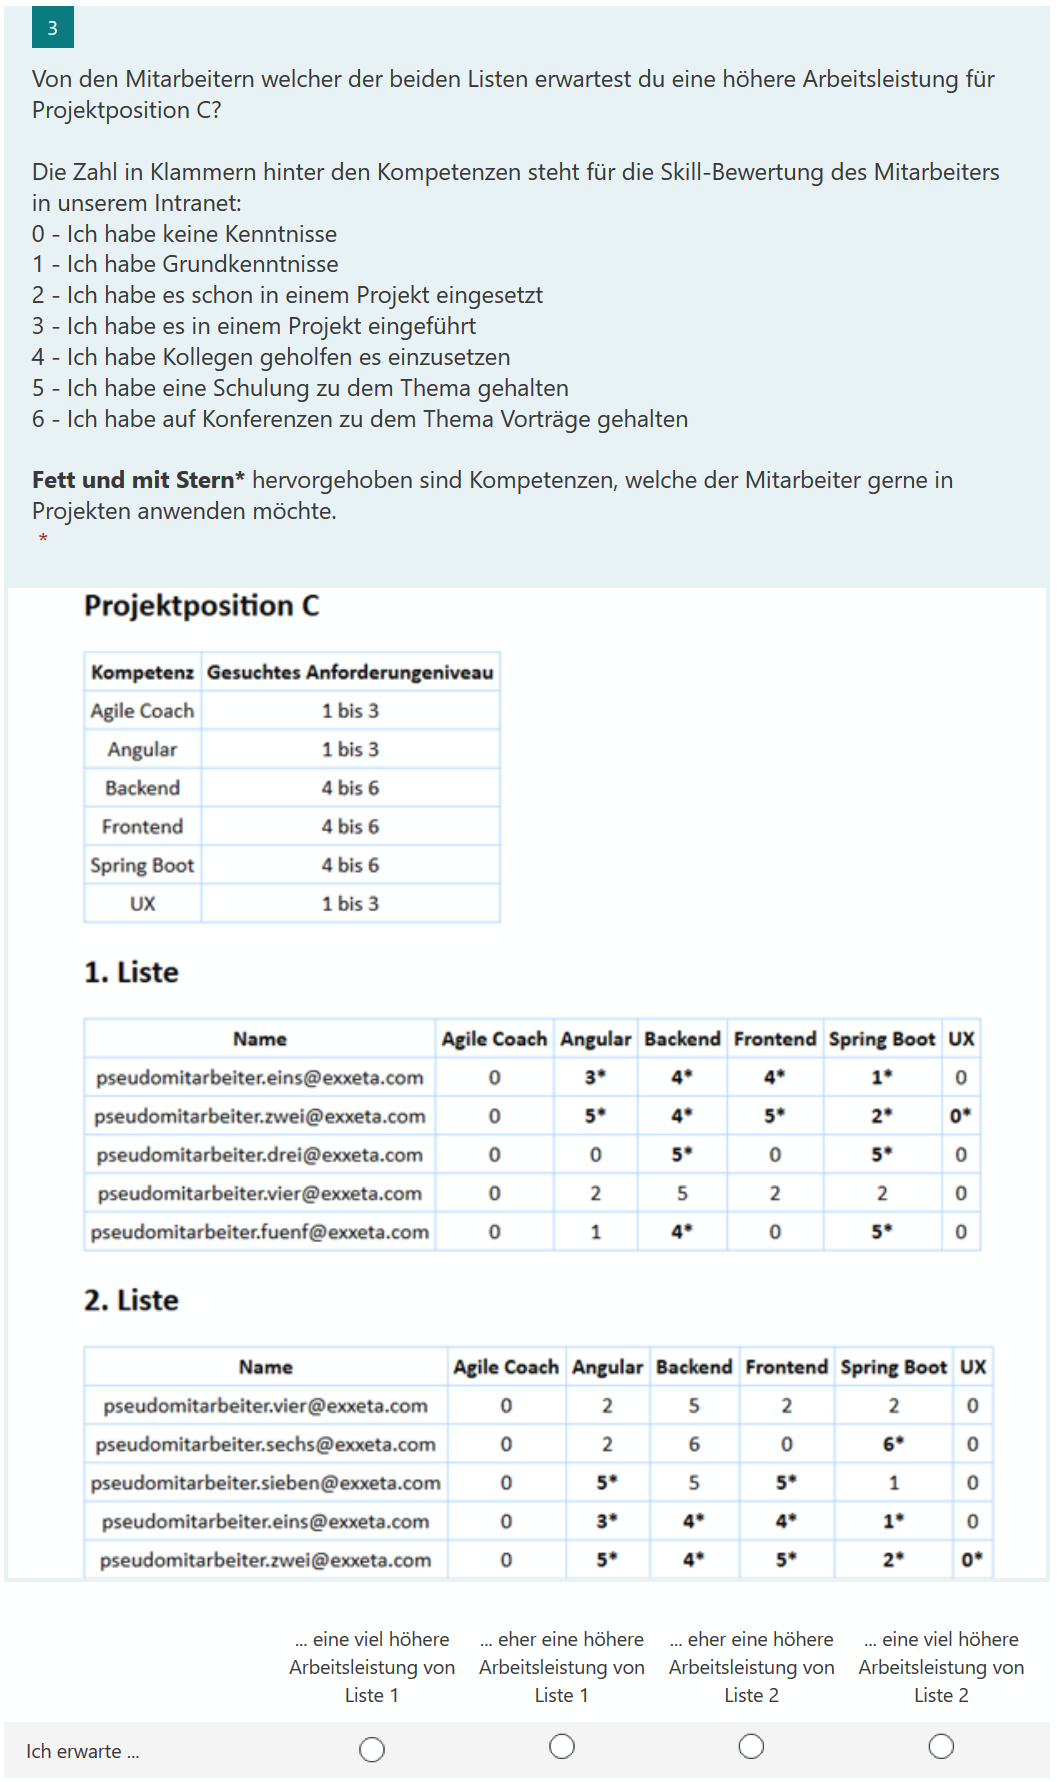
\includegraphics[width=1\textwidth]{gfx/projekt-c-liste-pseudonym.png}
\caption[Frage zur Bewertung der unterschiedlichen Listen]{Frage zur Bewertung der unterschiedlichen Listen\\
	(Klarnamen wurden aus Datenschutzgründen nachträglich pseudonymisiert)}
\label{fig:methodik:evaluation:manager:abb1}
\end{figure}
\shorthandon{"}
